\documentclass[tikz,border=5pt]{standalone}
\usepackage{amsmath,amssymb}
\usetikzlibrary{arrows.meta,decorations.markings,calc,backgrounds}

\begin{document}
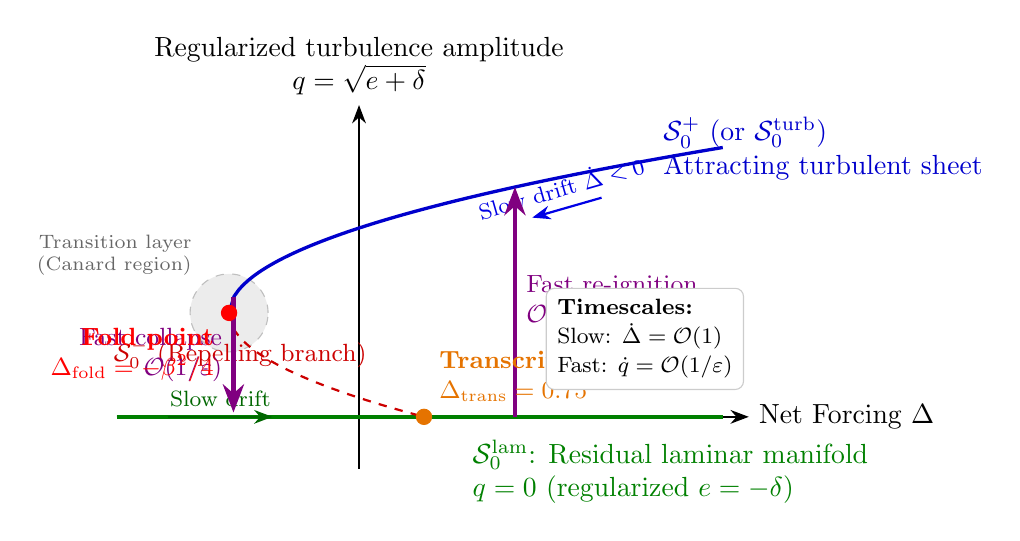
\begin{tikzpicture}[scale=1.1, >=Stealth]

    % --- Key Coordinates ---
    \coordinate (Fold) at (-1.5, 1.2);
    \coordinate (Transcritical) at (0.75, 0);

    % --- 1. Transition / Canard Region (Background Layer) ---
    \begin{scope}[on background layer]
        \filldraw[fill=gray!15, draw=gray!50, dashed] (Fold) circle (0.45);
        \node[gray!80!black, font=\scriptsize, align=right, above left=10pt] at (Fold)
            {Transition layer\\(Canard region)};
    \end{scope}

    % --- 2. Axes ---
    \draw[->, thick] (-2.8, 0) -- (4.5, 0) node[right] {Net Forcing $\Delta$};
    \draw[->, thick] (0, -0.6) -- (0, 3.6) node[above, align=center] {Regularized turbulence amplitude\\$q = \sqrt{e+\delta}$};

    % --- 3. Attracting Laminar Manifold S_0^lam (q = 0) ---
    \draw[very thick, green!50!black] (-2.8, 0) -- (4.2, 0);
    \node[green!50!black, below right, align=left] at (1.2, -0.15)
        {$\mathcal{S}_0^{\mathrm{lam}}$: Residual laminar manifold\\$q=0$ (regularized $e=-\delta$)};

    % --- 4. Repelling Branch S_0^- (Dashed Red, Fold to Transcritical) ---
    \draw[thick, dashed, red!80!black, domain=-1.5:0.75, samples=60]
        plot ({\x}, {1.2 - 0.8*sqrt(\x + 1.5)});
    \node[red!80!black, above left, font=\small] at (0.2, 0.45)
        {$\mathcal{S}_0^-$ (Repelling branch)};

    % --- 5. Attracting Turbulent Manifold S_0^+ (Solid Blue) ---
    \draw[very thick, blue!80!black, domain=-1.5:4.2, samples=100]
        plot ({\x}, {1.2 + 0.8*sqrt(\x + 1.5)});
    \node[blue!80!black, right, align=left] at (3.4, 3.1)
        {$\mathcal{S}_0^+$ (or $\mathcal{S}_0^{\mathrm{turb}}$)\\Attracting turbulent sheet};

    % --- 6. Slow Flow Dynamics (Tangent Drift along Attracting Sheets) ---
    % Slow cooling drift leftward along S_0^+ towards fold
    \draw[->, thick, blue!90!black] (2.8, 2.53) -- (2.0, 2.30)
        node[midway, above, sloped, font=\footnotesize] {Slow drift $\dot{\Delta} < 0$};
    % Slow momentum recovery drift rightward along S_0^lam
    \draw[->, thick, green!40!black] (-2.2, 0) -- (-1.0, 0)
        node[midway, above, font=\footnotesize] {Slow drift};

    % --- 7. Fast Subsystem Dynamics (Exact Vertical Jumps) ---
    % Fast Collapse past the fold (at \Delta = -1.45, starting on S_0^+)
    \pgfmathsetmacro{\qcollapse}{1.2 + 0.8*sqrt(-1.45 + 1.5)}
    \draw[->, ultra thick, violet] (-1.45, \qcollapse) -- (-1.45, 0.05)
        node[midway, left, align=right, font=\small] {Fast collapse\\$\mathcal{O}(1/\varepsilon)$};

    % Fast Re-ignition past the separatrix (at \Delta = 1.8, ending on S_0^+)
    \pgfmathsetmacro{\qreignite}{1.2 + 0.8*sqrt(1.8 + 1.5)}
    \draw[->, ultra thick, violet] (1.8, 0.0) -- (1.8, \qreignite)
        node[midway, right, align=left, font=\small] {Fast re-ignition\\$\mathcal{O}(1/\varepsilon)$};

    % --- 8. Critical Points (Bifurcations) ---
    % Fold Point
    \filldraw[red] (Fold) circle (2.5pt)
        node[below left=2pt, align=right, font=\small]
        {\textbf{Fold point}\\$\Delta_{\mathrm{fold}} = -\beta^2/4$};

    % Transcritical Point
    \filldraw[orange!90!black] (Transcritical) circle (2.5pt)
        node[above right=2pt, align=left, font=\small]
        {\textbf{Transcritical point}\\$\Delta_{\mathrm{trans}} = 0.75$};

    % --- 9. Timescale Box ---
    \node[draw=gray!40, fill=white, rounded corners=3pt, inner sep=4pt, align=left, font=\footnotesize]
        at (3.3, 0.9) {
            \textbf{Timescales:}\\[1pt]
            Slow: $\dot{\Delta} = \mathcal{O}(1)$\\[1pt]
            Fast: $\dot{q} = \mathcal{O}(1/\varepsilon)$
        };

\end{tikzpicture}
\end{document}
